\subsection{Identifikationssysteme (Scanner)}
\subsubsection{Allgemeine Einordnung}
Die eindeutige Identifikation von Bauteilen ist ein grundlegender Bestandteil logistischer Prozesse. Diese Identifikation kiann über unterschiedlichste Verfahren erfolgen. Die gängigste Prüfung erfolgt durch \textbf{Scanner}.\\
Automatisierte Systeme benötigen eine klare Zuordnung von Objekten um richtig arbeiten zu können. In der Logistik ist dies von besonders hoher Bedeutung.\\
Ohne eine solche Identifikation ist keine auftragsbasierte Steuerung möglich und es kann zu erheblichen Komplikationen kommen.
\subsubsection{Scanner als Identifikationssystem}

Die Aufgabe eines Einlesegerätes besteht darin, Daten schnell und zuverlässig zu erfassen. Zum Einlesen beziehungsweise zur Eingabe von Daten stehen verschiedene Möglichkeiten zur Verfügung:
\begin{itemize}
	\item Eingabe über Tastatur 
	\item Einlesen über ein Scan-Gerät
	\item Erkennung des Bauteils über eine Kamera
\end{itemize}

Im Logistikbereich müssen Daten in der Regel schnell und fehlerfrei übertragen werden. Für diese Anwendung eignen sich Scanner besonders gut. Diese sind einfach in der Handhabung und ermöglichen eine schnelle Erfassung von Daten. Im Gegensatz zur Eingabe über die Tastatur ist keine manuelle Eingabe erforderlich, wodurch Fehler reduziert werden können.\\

Zur Identifikation werden Codierungen benötigt. In der Regel werden hierfür Barcodes oder QR-Codes verwendet.\\
Im Folgenden ist eine Übersicht über die wichtigsten Merkmale und Unterschiede von \textbf{QR-Codes} und \textbf{Barcodes} dargestellt:

\begin{table}[H]
	\centering
	\renewcommand{\arraystretch}{1.3}
	\begin{tabular}{|p{4cm}|p{4.5cm}|p{4.5cm}|}
		\hline
		\textbf{Merkmal} & \textbf{Barcode} & \textbf{QR-Code} \\ \hline
		Struktur & Eindimensional (1D) & Zweidimensional (2D) \\ \hline
		Datenspeicher & Geringe Datenmenge & Hohe Datenmenge \\ \hline
		Leserichtung & Nur horizontal lesbar & Aus allen Richtungen lesbar \\ \hline
		Fehlerkorrektur & Kaum vorhanden & Integrierte Fehlerkorrektur \\ \hline
		Verwendung & Artikeletiketten, Lager & Industrie, Tracking, Datenübertragung \\ \hline
		Informationsgehalt & Meist nur ID / Nummer & Kann komplexe Daten enthalten \\ \hline
	\end{tabular}
	\caption{Vergleich von Barcode- und QR-Code-Systemen; Quelle: \cite{Codes}}
	\label{tab:Codes}
\end{table}

In Tabelle \ref{tab:Codes} werden die wesentlichen Unterschiede zwischen Barcode- und QR-Code-Systemen dargestellt. Während Barcodes aufgrund ihrer einfachen Struktur hauptsächlich zur Identifikation von Artikeln verwendet werden, bieten QR-Codes aufgrund ihres zweidimensionalen Aufbaus die Möglichkeit, deutlich mehr Informationen zu speichern.\\

Für industrielle Anwendungen, wie beispielsweise in automatisierten Lagersystemen, werden in vielen Fällen weiterhin Barcodes eingesetzt, da diese für die eindeutige Identifikation von Bauteilen ausreichend sind und sich durch eine einfache Implementierung auszeichnen. In komplexeren Anwendungen können jedoch auch QR-Codes verwendet werden, insbesondere wenn \subsubsection{Funktionsweise eines Scanners}

Der Einlesevorgang bei einem Scanner erfolgt über ein optisches Verfahren, welches je nach Bauart auf Licht-, Laser- oder Kameratechnologie basiert. 
Beim Lichtverfahren wird das Objekt gleichmäßig ausgeleuchtet, während beim Laserverfahren ein gebündelter Lichtstrahl über den Code geführt wird. Kamerabasierte Systeme arbeiten hingegen mit Bildsensoren und erfassen den Code flächenhaft.\\

Allen Verfahren gemeinsam ist die Auswertung von Hell-Dunkel-Unterschieden, welche die codierten Informationen repräsentieren.\\

Der Ablauf des Einlesevorgangs lässt sich wie folgt beschreiben:
\begin{itemize}
	\item 1. Beleuchtung des Codes durch Licht- oder Laserquelle
	\item 2. Erfassung der reflektierten Lichtanteile durch einen Sensor
	\item 3. Unterscheidung zwischen hellen und dunklen Bereichen des Codes
	\item 4. Umwandlung der optischen Signale in elektrische Signale
	\item 5. Verarbeitung und Interpretation als Zahlen- oder Zeichenfolge
\end{itemize}

Die erzeugte Zeichenfolge entspricht dabei der im Code enthaltenen Information, beispielsweise einer Artikelnummer oder Bauteilkennung. Diese kann anschließend von nachgelagerten Systemen weiterverarbeitet werden.

\begin{figure}[H]
	\centering
	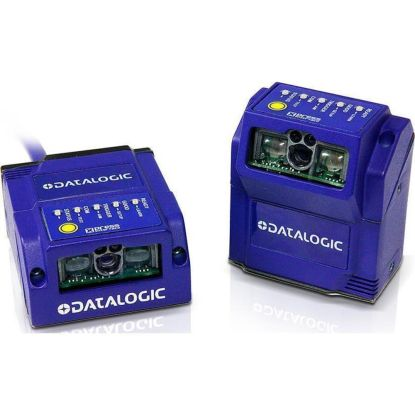
\includegraphics[width=0.3\textwidth]{images/Matrix200.jpg}
	\caption{Kamerabasierter Scanner\cite{Datalogic}}
	\label{fig:MatrixGrundlagen}
\end{figure}
\subsubsection{Datenübertragung / Schnittstelle}

Die Datenübertragung erfolgt in der Regel seriell an ein übergeordnetes System. Die erfassten Daten werden unmittelbar nach dem Einlesevorgang an die Steuerung, beispielsweise einen PC oder eine SPS, weitergeleitet. Die Ausgabe erfolgt üblicherweise als Zeichenkette (String).\\
Je nach Datenformat sind Anpassungen innerhalb der Steuerung oder durch eine zwischengeschaltete Software erforderlich, um eine korrekte Weiterverarbeitung der Daten zu gewährleisten. Am Ende des Scanwertes befindet sich in der Regel ein Abschlusszeichen, beispielsweise \texttt{"\textbackslash n"} oder ein "\texttt{Enter"}-Signal.\\

Die \textbf{Schnittstelle} kann je nach Scannerart unterschiedlich ausgeführt sein. Häufig werden RS232 sowie USB verwendet. Während RS232 eine klassische serielle Schnittstelle darstellt, kann USB durch die Emulation eines virtuellen COM-Ports ebenfalls wie eine serielle Schnittstelle verwendet werden.\\

Im Folgenden sind die wichtigsten Eigenschaften und Unterschiede beider Anschlussarten dargestellt:

\begin{table}[H]
	\centering
	\renewcommand{\arraystretch}{1.3}
	\begin{tabular}{|p{4cm}|p{4.5cm}|p{4.5cm}|}
		\hline
		\textbf{Merkmal} & \textbf{RS232} & \textbf{USB} \\ \hline
		Übertragungsart & Klassisch seriell & Paketbasiert (virtuell seriell möglich) \\ \hline
		Schnittstelle & Physischer COM-Port & Virtueller COM-Port (häufig) \\ \hline
		Datenrate & Niedrig bis mittel & Hoch \\ \hline
		Verzögerung & Sehr gering & Gering \\ \hline
		Implementierung & Einfach, robust & Etwas komplexer \\ \hline
		Verwendung & Industrie / Automatisierung & PC-Systeme / moderne Geräte \\ \hline
	\end{tabular}
	\caption{Vergleich der Schnittstellen RS232\cite{rs232_mikrocontroller} und USB\cite{usb_standard}}
	\label{tab:schnittstellen}
\end{table}

Aus Tabelle \ref{tab:schnittstellen} wird deutlich, dass beide Schnittstellen ihre Berechtigung im industriellen Umfeld besitzen. Während RS232 besonders durch seine einfache und robuste Struktur überzeugt\cite{rs232_mikrocontroller}, bietet USB eine höhere Datenübertragungsrate und wird häufig durch virtuelle COM-Ports in bestehende Systeme integriert\cite{usb_standard}.\\

Schlussendlich werden die erfassten Daten über eine Programmanwendung, beispielsweise in Python oder C, weiterverarbeitet. Dabei können projektabhängige Anpassungen vorgenommen werden, um die Daten entsprechend aufzubereiten. Die eigentliche Prozesslogik wird somit softwareseitig realisiert, wodurch automatisierte Abläufe, wie beispielsweise die Zuordnung von Bauteilen anhand von Scanwerten, angestoßen werden können.\clearpage
\subsubsection{Vorteile beim Einsatz eines Scanners}

Der Einsatz von Scannern bietet insbesondere im industriellen und logistischen Umfeld zahlreiche Vorteile. Im Folgenden sind die wichtigsten Aspekte übersichtlich dargestellt:

\begin{table}[H]
	\centering
	\renewcommand{\arraystretch}{1.3}
	\begin{tabular}{|p{5cm}|p{7cm}|}
		\hline
		\textbf{Vorteil} & \textbf{Beschreibung} \\ \hline
		Schnelle Datenerfassung & Scanvorgänge erfolgen in sehr kurzer Zeit und ermöglichen hohe Prozessgeschwindigkeiten \\ \hline
		Reduzierte Fehlerquote & Keine manuelle Eingabe notwendig, dadurch geringere Eingabefehler \\ \hline
		Einfache Integration & Scanner lassen sich leicht in bestehende Systeme einbinden \\ \hline
		Hohe Zuverlässigkeit & Robuste Technik, geeignet für industrielle Anwendungen \\ \hline
		Automatisierungspotenzial & Ermöglicht die direkte Weiterverarbeitung von Daten in automatisierten Prozessen \\ \hline
		Eindeutige Identifikation & Barcodes und QR-Codes ermöglichen klare Zuordnung von Bauteilen \\ \hline
		Flexibilität & Einsetzbar in verschiedenen Anwendungen und Branchen \\ \hline
	\end{tabular}
	\caption{Vorteile des Einsatzes von Scannern in automatisierten Systemen\cite{Datalogic}}
	\label{tab:vorteile_scanner}
\end{table}

Wie in Tabelle \ref{tab:vorteile_scanner} dargestellt, tragen Scanner maßgeblich zur Effizienzsteigerung in automatisierten Prozessen bei. Insbesondere die schnelle und fehlerarme Datenerfassung stellt einen entscheidenden Vorteil dar. Im Zusammenspiel mit softwarebasierten Verarbeitungssystemen können somit vollständig automatisierte Abläufe realisiert werden.